\documentclass[11pt]{article}
\usepackage[textwidth=18.0cm, textheight=23.0cm, top=2.0cm]{geometry}
\usepackage{pst-all}
\usepackage{amssymb}
\usepackage{tikz}
\usepackage{underscore}\begin{document}
\pagestyle{empty}


ClassName: \underline{\textbf{Class_05.2bp-28}}
\par
BinSize: \underline{\textbf{100 × 100}}
\par
ReduceSize: \underline{\textbf{100 × 100}}
\par
TypeNum: \underline{\textbf{60}}
\par
Num: \underline{\textbf{60}}
\par
OutS: \underline{\textbf{160000}}
\par
InS: \underline{\textbf{145150}}
\par
Rate: \underline{\textbf{0.907}}
\par
UB: \underline{\textbf{16}}
\par
LB0: \underline{\textbf{16}}
\par
LB: \underline{\textbf{16}}
\par
LBWithCut: \underline{\textbf{16}}
\par
NodeCut: \underline{\textbf{0}}
\par
ExtendedNodeCnt: \underline{\textbf{1}}
\par
GenNodeCnt: \underline{\textbf{1}}
\par
PrimalNode: \underline{\textbf{0}}
\par
ColumnCount: \underline{\textbf{16}}
\par
TotalCutCount: \underline{\textbf{0}}
\par
RootCutCount: \underline{\textbf{0}}
\par
LPSolverCnt: \underline{\textbf{1}}
\par
PricingSolverCnt: \underline{\textbf{0}}
\par
BranchAndBoundNum: \underline{\textbf{1}}
\par
isOpt: \underline{\textbf{true}}
\par
TimeOnInitSolution: \underline{\textbf{0.360 s}}
\par
TimeOnPrimal: \underline{\textbf{0.000 s}}
\par
TimeOnPricing: \underline{\textbf{0.000 s}}
\par
TimeOnRmp: \underline{\textbf{0.063 s}}
\par
TotalTime: \underline{\textbf{0.485 s}}
\par
\newpage


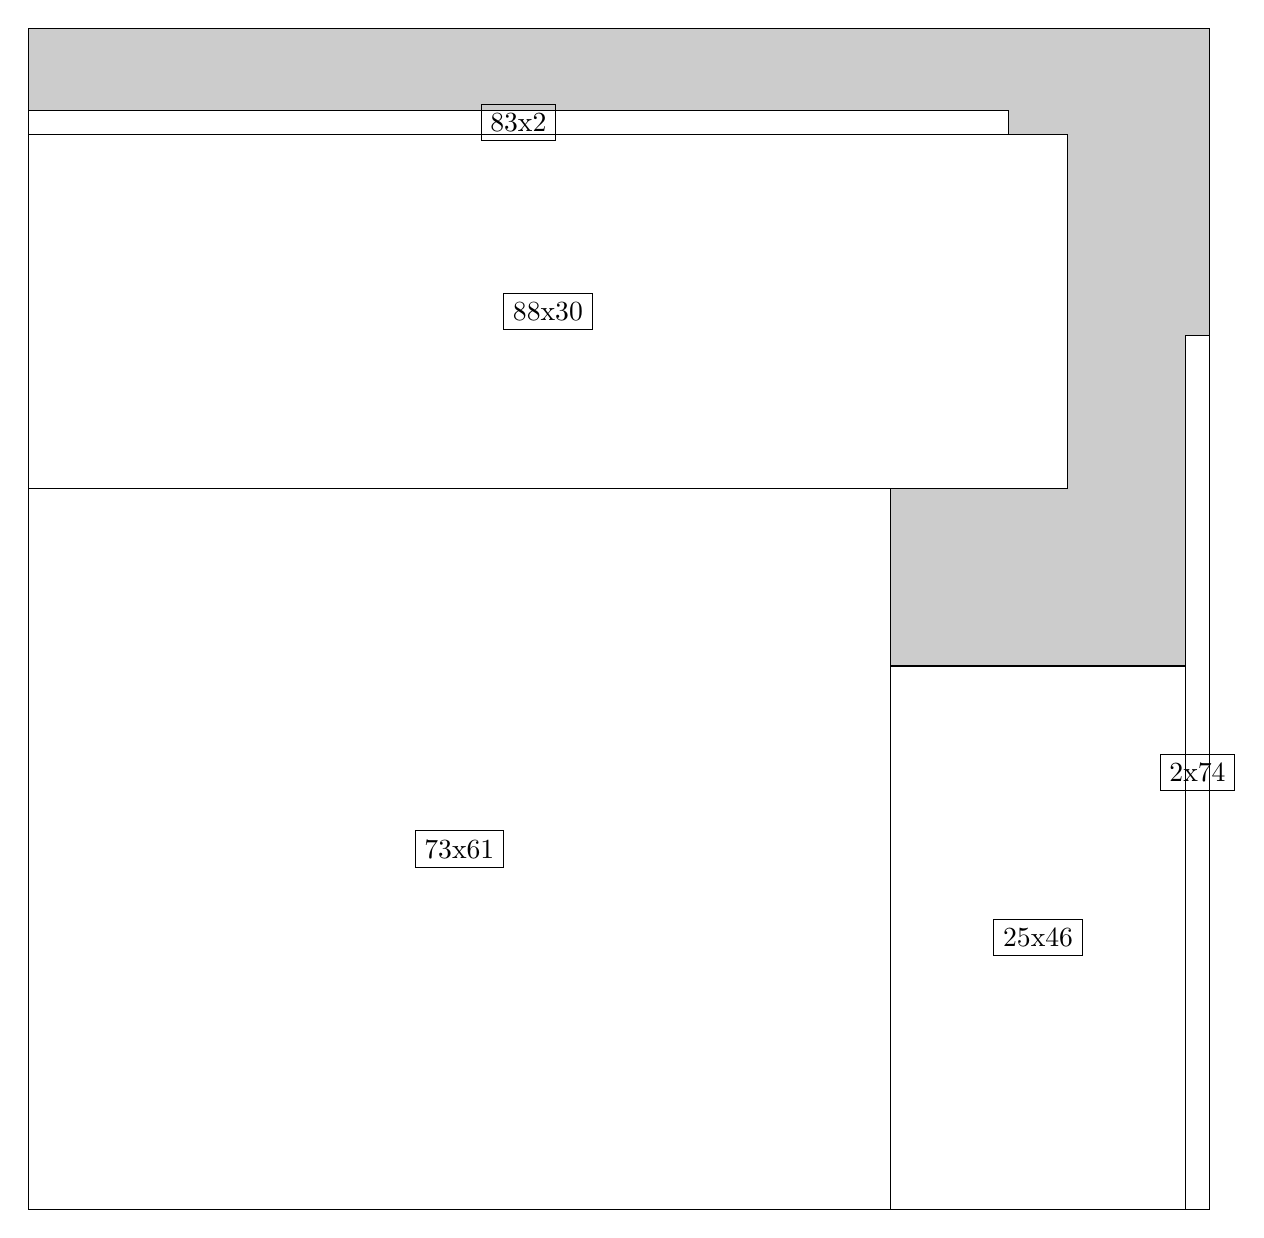
\begin{tikzpicture}[shorten >=1pt,scale=1.0,every node/.style={scale=1.0},->]
\tikzstyle{vertex}=[circle,fill=black!25,minimum size=14pt,inner sep=0pt]
\filldraw[fill=gray!40!white, draw=black] (0,0) rectangle (15.0,15.0);
\foreach \name/\x/\y/\w/\h in {25x46/10.95/0.0/3.75/6.8999999999999995,73x61/0.0/0.0/10.95/9.15,88x30/0.0/9.15/13.2/4.5,83x2/0.0/13.65/12.45/0.3,2x74/14.7/0.0/0.3/11.1}
\filldraw[fill=white!40!white, draw=black] (\x,\y) rectangle node[draw] (\name) {\name} ++(\w,\h);
\end{tikzpicture}


w =25 , h =46 , x =73 , y =0 , v =1150
\par
w =73 , h =61 , x =0 , y =0 , v =4453
\par
w =88 , h =30 , x =0 , y =61 , v =2640
\par
w =83 , h =2 , x =0 , y =91 , v =166
\par
w =2 , h =74 , x =98 , y =0 , v =148
\par
\newpage


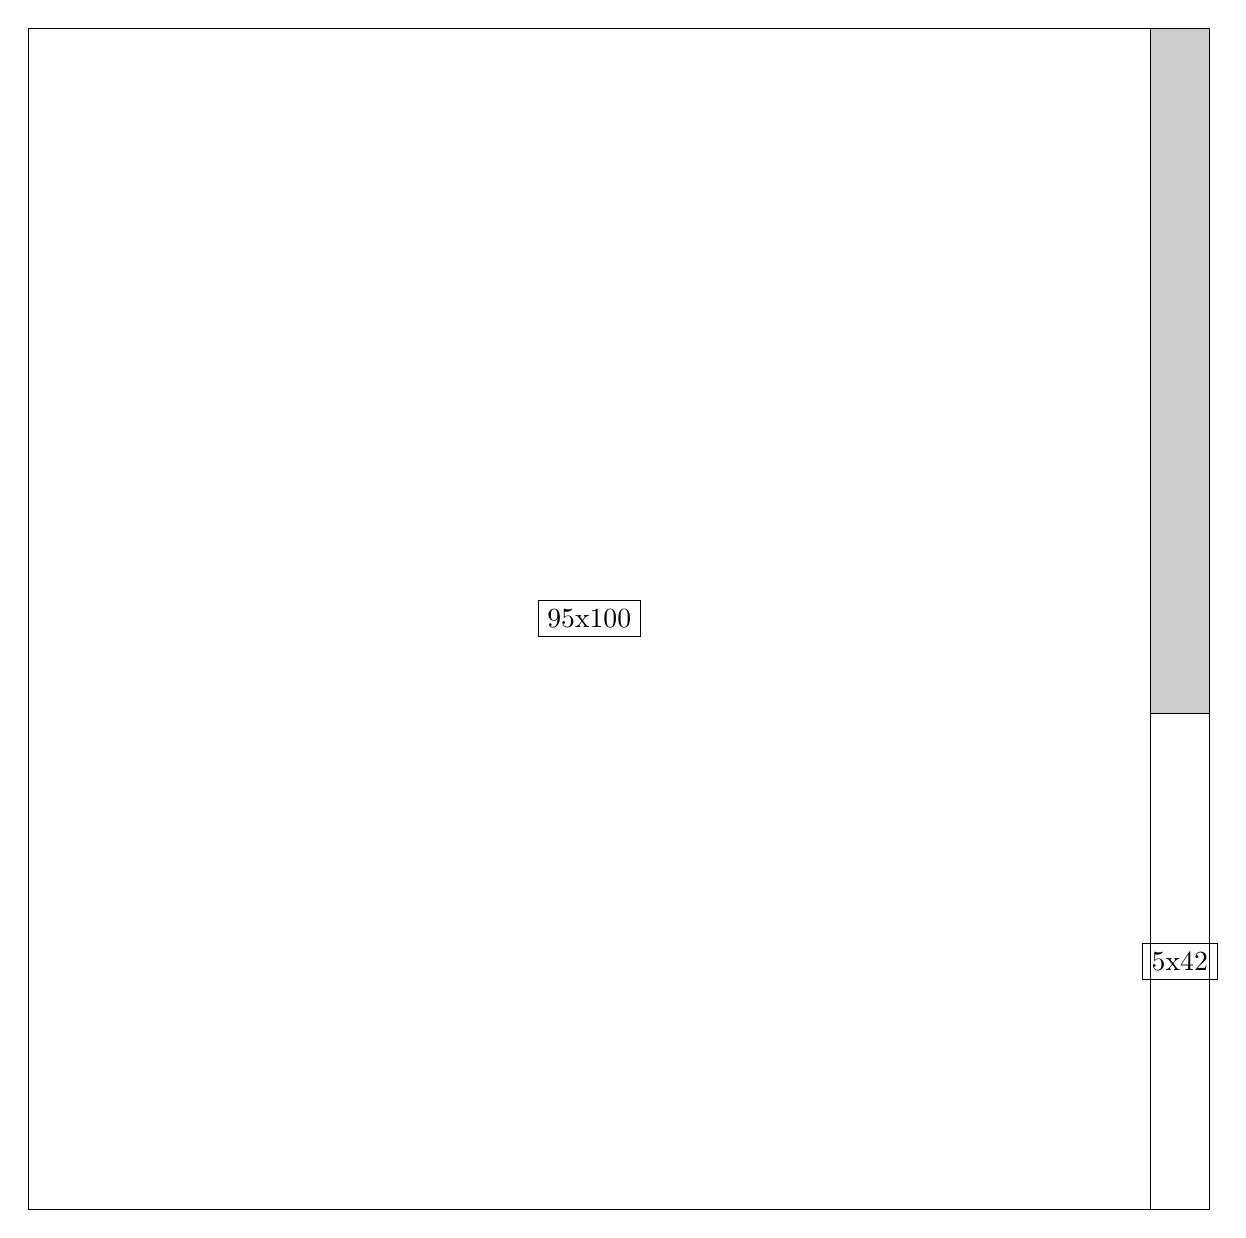
\begin{tikzpicture}[shorten >=1pt,scale=1.0,every node/.style={scale=1.0},->]
\tikzstyle{vertex}=[circle,fill=black!25,minimum size=14pt,inner sep=0pt]
\filldraw[fill=gray!40!white, draw=black] (0,0) rectangle (15.0,15.0);
\foreach \name/\x/\y/\w/\h in {95x100/0.0/0.0/14.25/15.0,5x42/14.25/0.0/0.75/6.3}
\filldraw[fill=white!40!white, draw=black] (\x,\y) rectangle node[draw] (\name) {\name} ++(\w,\h);
\end{tikzpicture}


w =95 , h =100 , x =0 , y =0 , v =9500
\par
w =5 , h =42 , x =95 , y =0 , v =210
\par
\newpage


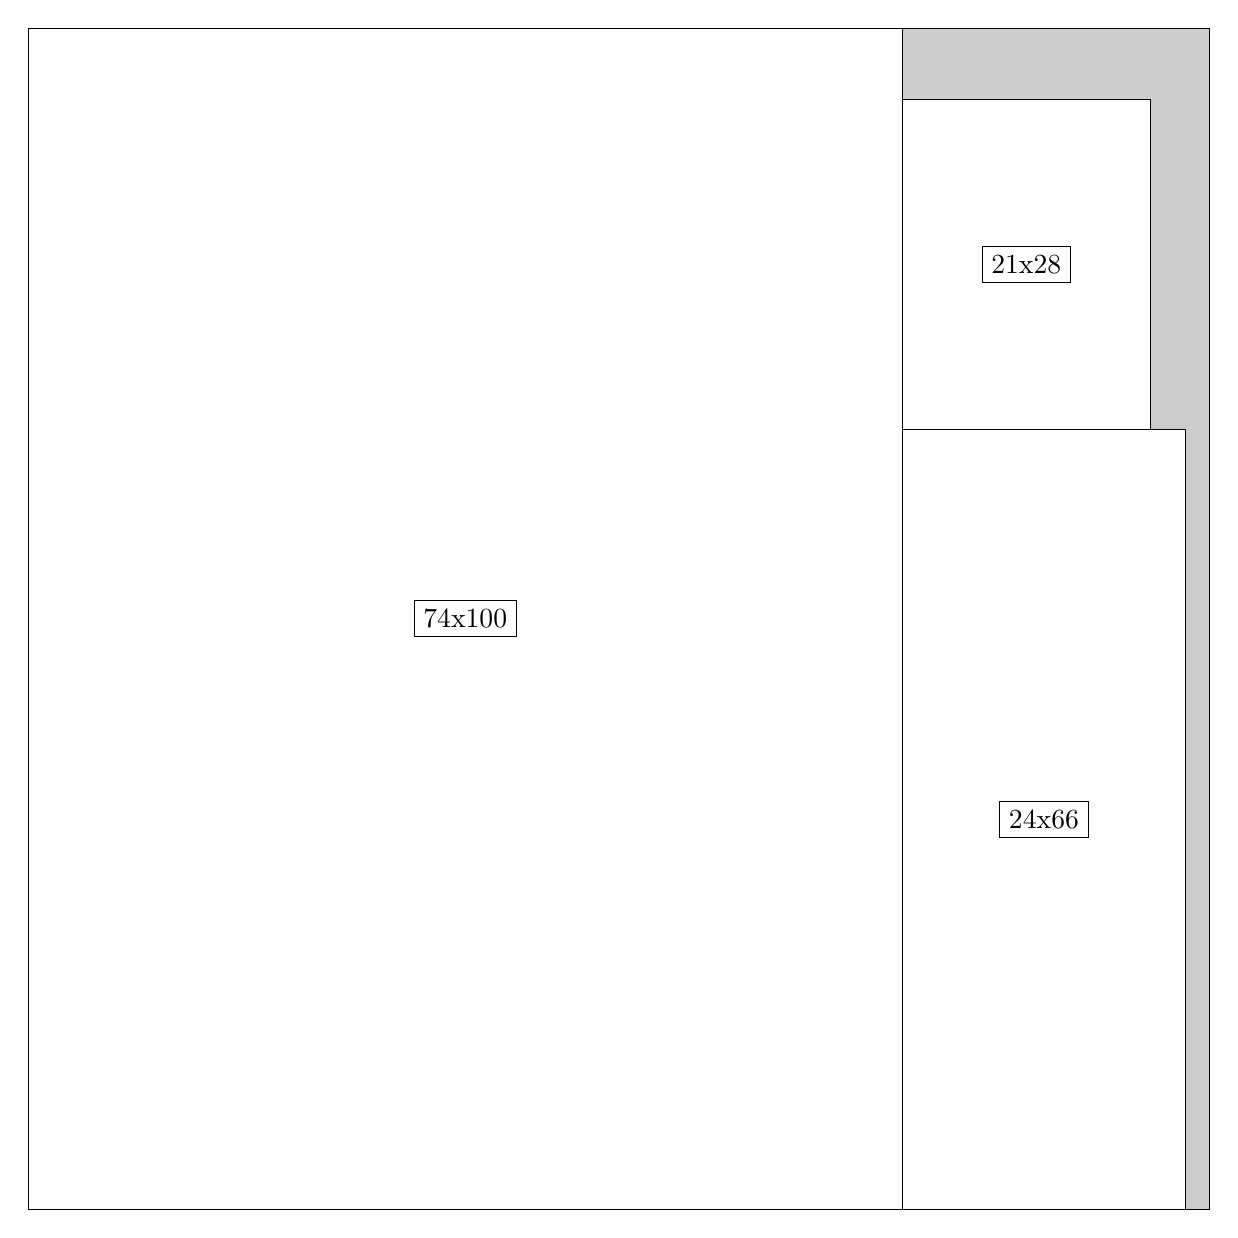
\begin{tikzpicture}[shorten >=1pt,scale=1.0,every node/.style={scale=1.0},->]
\tikzstyle{vertex}=[circle,fill=black!25,minimum size=14pt,inner sep=0pt]
\filldraw[fill=gray!40!white, draw=black] (0,0) rectangle (15.0,15.0);
\foreach \name/\x/\y/\w/\h in {74x100/0.0/0.0/11.1/15.0,24x66/11.1/0.0/3.5999999999999996/9.9,21x28/11.1/9.9/3.15/4.2}
\filldraw[fill=white!40!white, draw=black] (\x,\y) rectangle node[draw] (\name) {\name} ++(\w,\h);
\end{tikzpicture}


w =74 , h =100 , x =0 , y =0 , v =7400
\par
w =24 , h =66 , x =74 , y =0 , v =1584
\par
w =21 , h =28 , x =74 , y =66 , v =588
\par
\newpage


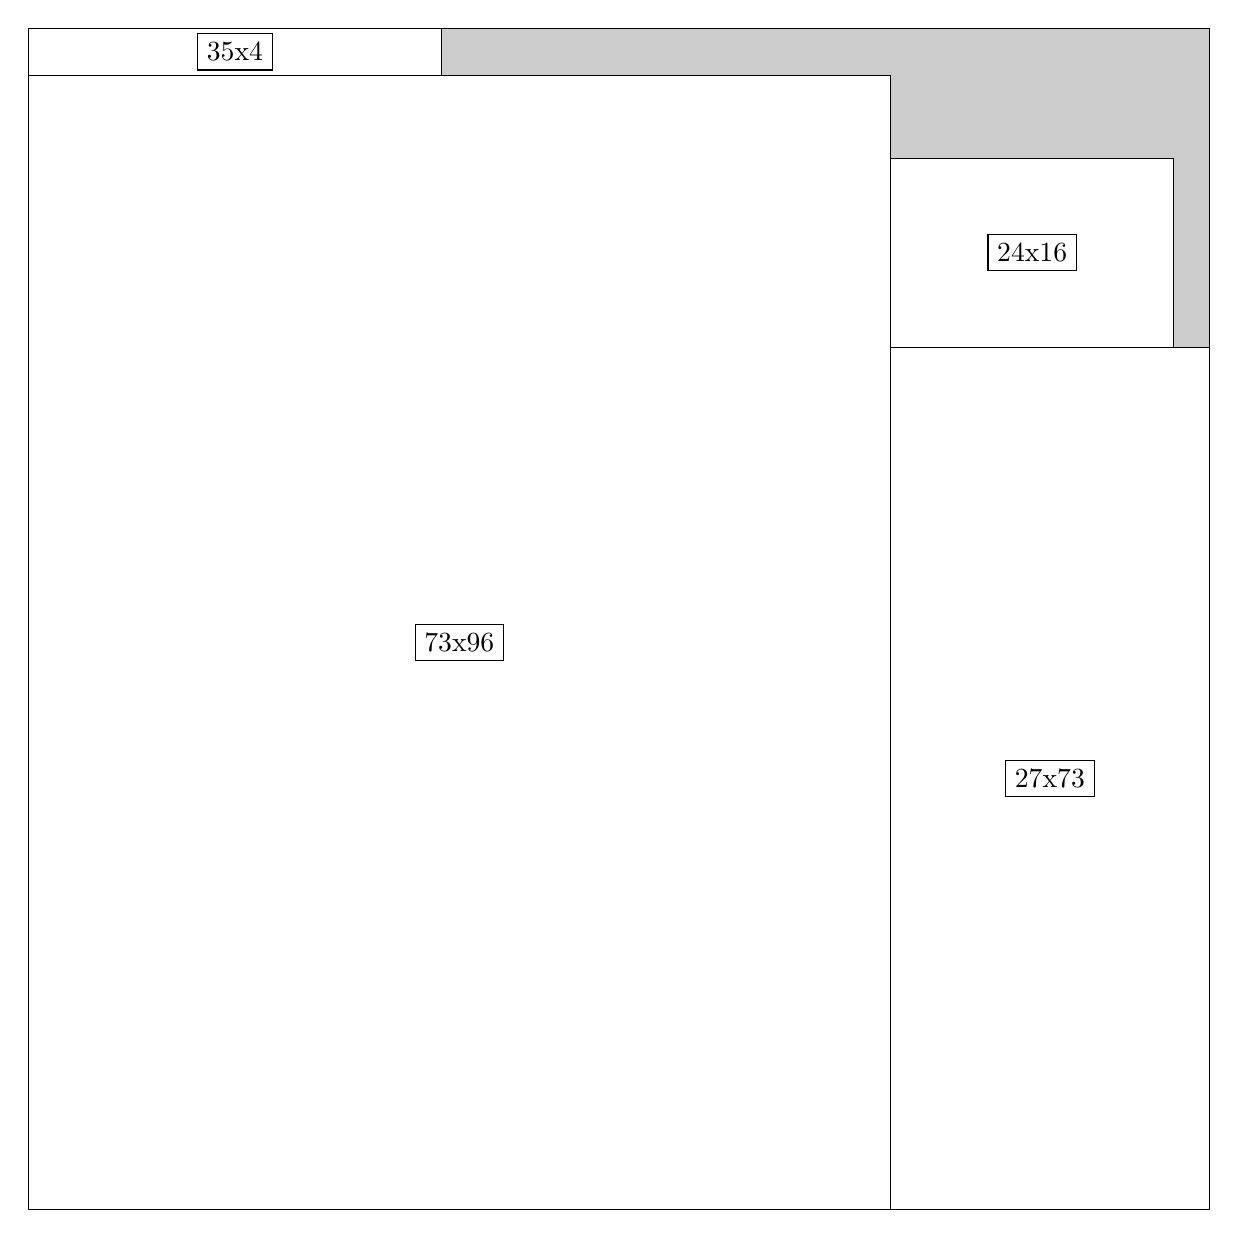
\begin{tikzpicture}[shorten >=1pt,scale=1.0,every node/.style={scale=1.0},->]
\tikzstyle{vertex}=[circle,fill=black!25,minimum size=14pt,inner sep=0pt]
\filldraw[fill=gray!40!white, draw=black] (0,0) rectangle (15.0,15.0);
\foreach \name/\x/\y/\w/\h in {73x96/0.0/0.0/10.95/14.399999999999999,27x73/10.95/0.0/4.05/10.95,24x16/10.95/10.95/3.5999999999999996/2.4,35x4/0.0/14.399999999999999/5.25/0.6}
\filldraw[fill=white!40!white, draw=black] (\x,\y) rectangle node[draw] (\name) {\name} ++(\w,\h);
\end{tikzpicture}


w =73 , h =96 , x =0 , y =0 , v =7008
\par
w =27 , h =73 , x =73 , y =0 , v =1971
\par
w =24 , h =16 , x =73 , y =73 , v =384
\par
w =35 , h =4 , x =0 , y =96 , v =140
\par
\newpage


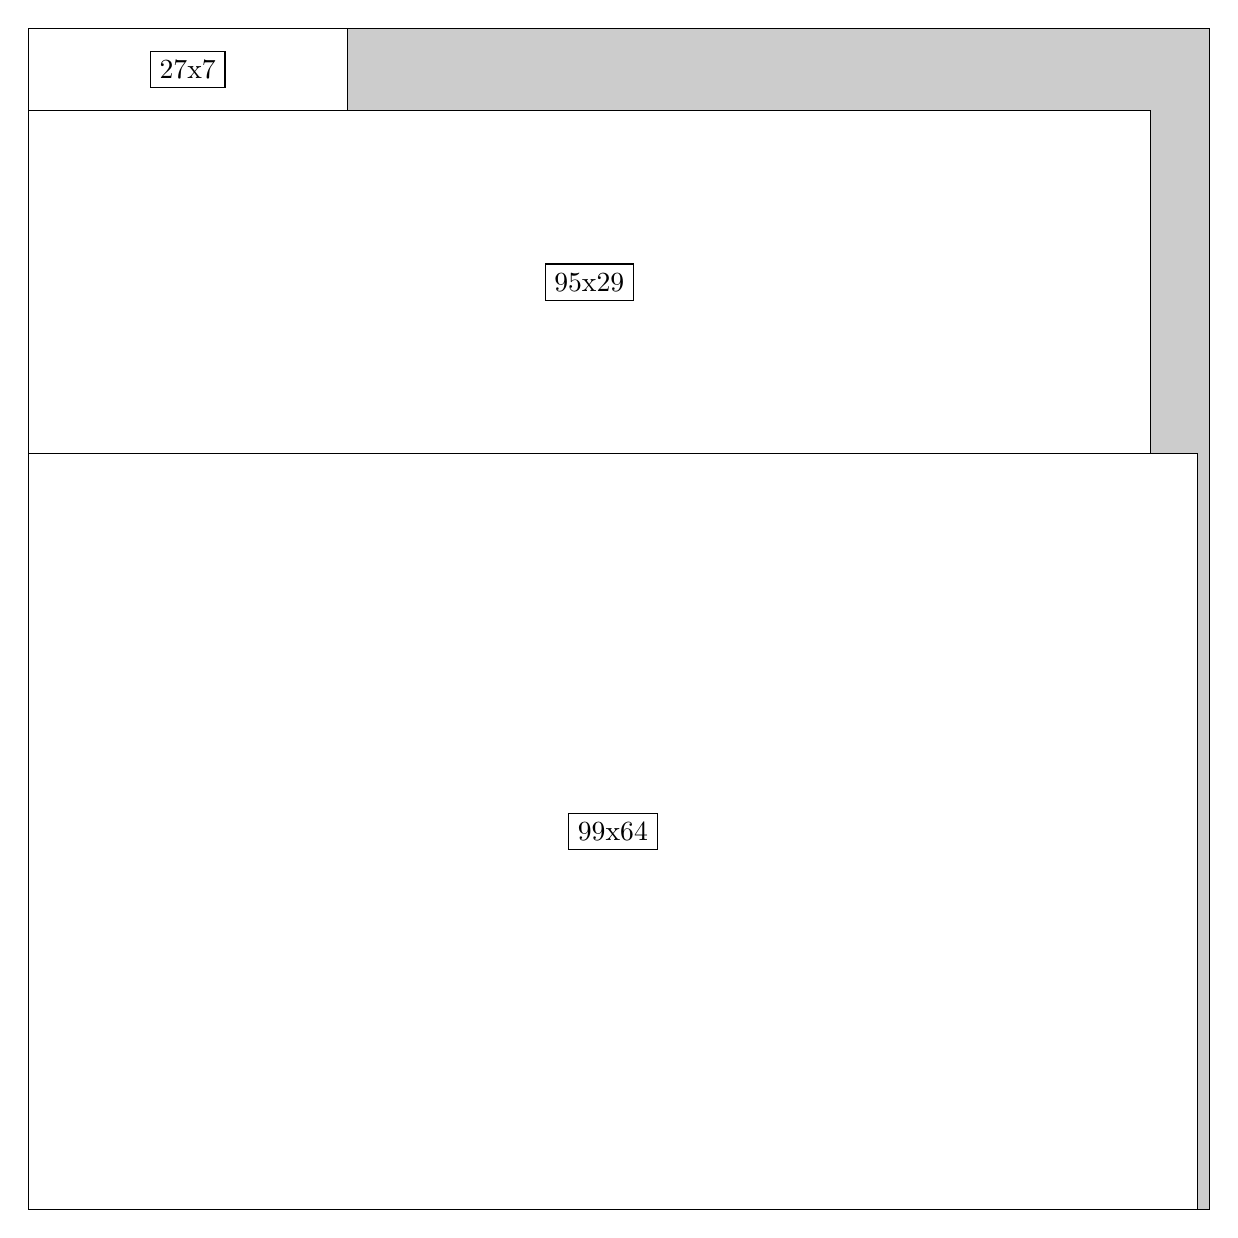
\begin{tikzpicture}[shorten >=1pt,scale=1.0,every node/.style={scale=1.0},->]
\tikzstyle{vertex}=[circle,fill=black!25,minimum size=14pt,inner sep=0pt]
\filldraw[fill=gray!40!white, draw=black] (0,0) rectangle (15.0,15.0);
\foreach \name/\x/\y/\w/\h in {99x64/0.0/0.0/14.85/9.6,95x29/0.0/9.6/14.25/4.35,27x7/0.0/13.95/4.05/1.05}
\filldraw[fill=white!40!white, draw=black] (\x,\y) rectangle node[draw] (\name) {\name} ++(\w,\h);
\end{tikzpicture}


w =99 , h =64 , x =0 , y =0 , v =6336
\par
w =95 , h =29 , x =0 , y =64 , v =2755
\par
w =27 , h =7 , x =0 , y =93 , v =189
\par
\newpage


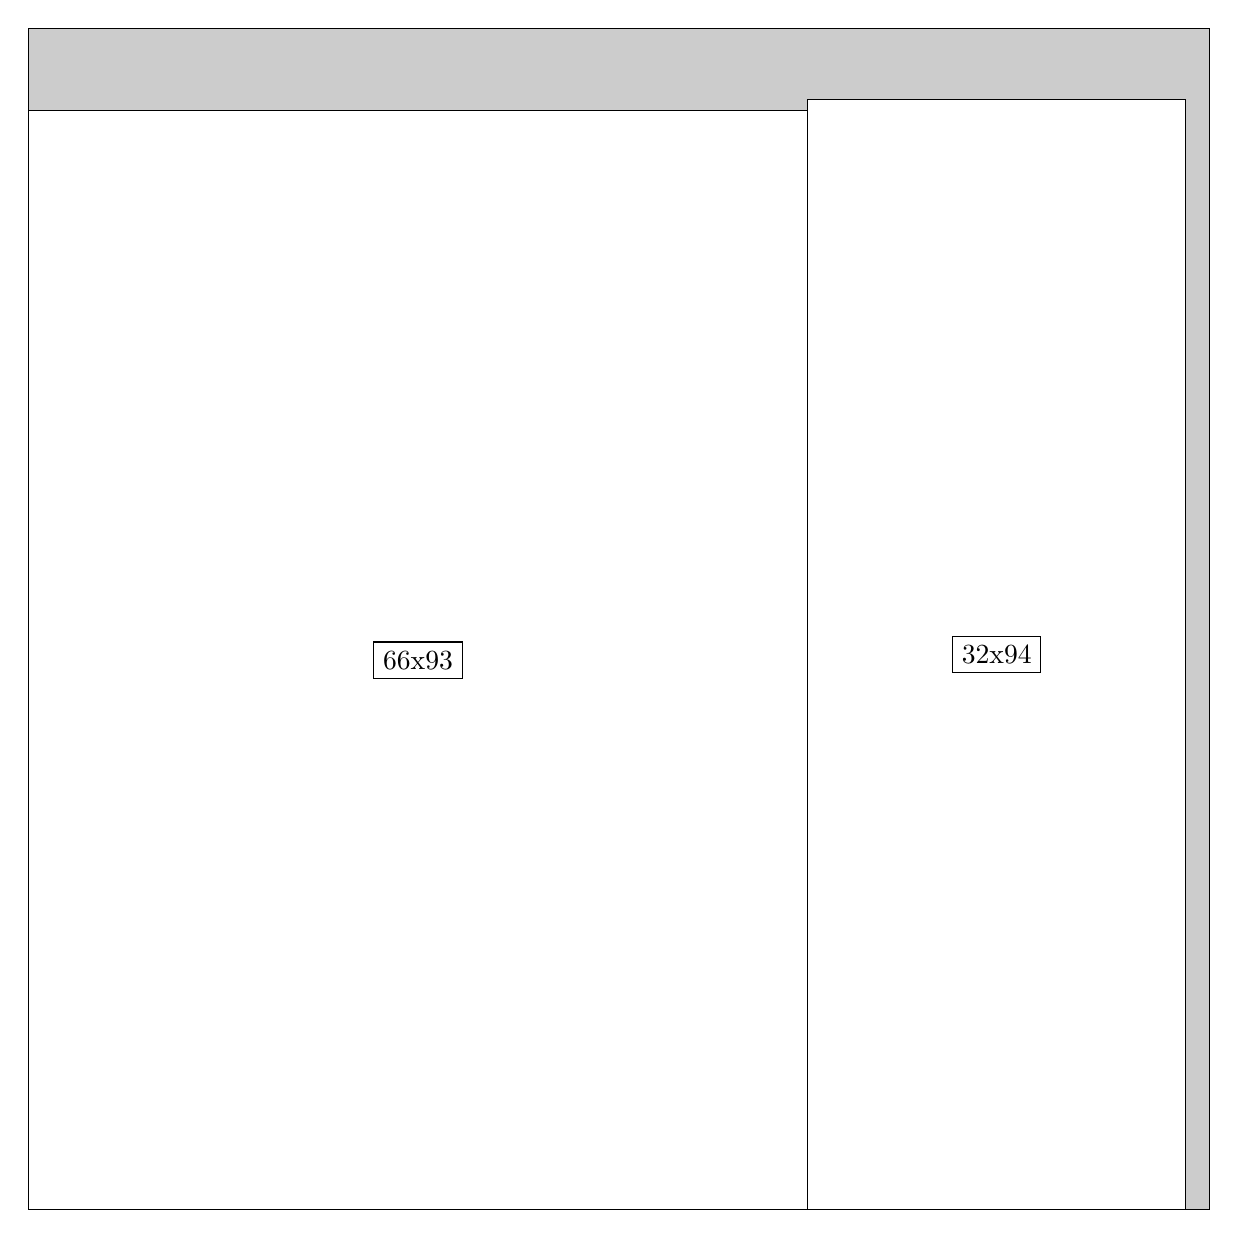
\begin{tikzpicture}[shorten >=1pt,scale=1.0,every node/.style={scale=1.0},->]
\tikzstyle{vertex}=[circle,fill=black!25,minimum size=14pt,inner sep=0pt]
\filldraw[fill=gray!40!white, draw=black] (0,0) rectangle (15.0,15.0);
\foreach \name/\x/\y/\w/\h in {66x93/0.0/0.0/9.9/13.95,32x94/9.9/0.0/4.8/14.1}
\filldraw[fill=white!40!white, draw=black] (\x,\y) rectangle node[draw] (\name) {\name} ++(\w,\h);
\end{tikzpicture}


w =66 , h =93 , x =0 , y =0 , v =6138
\par
w =32 , h =94 , x =66 , y =0 , v =3008
\par
\newpage


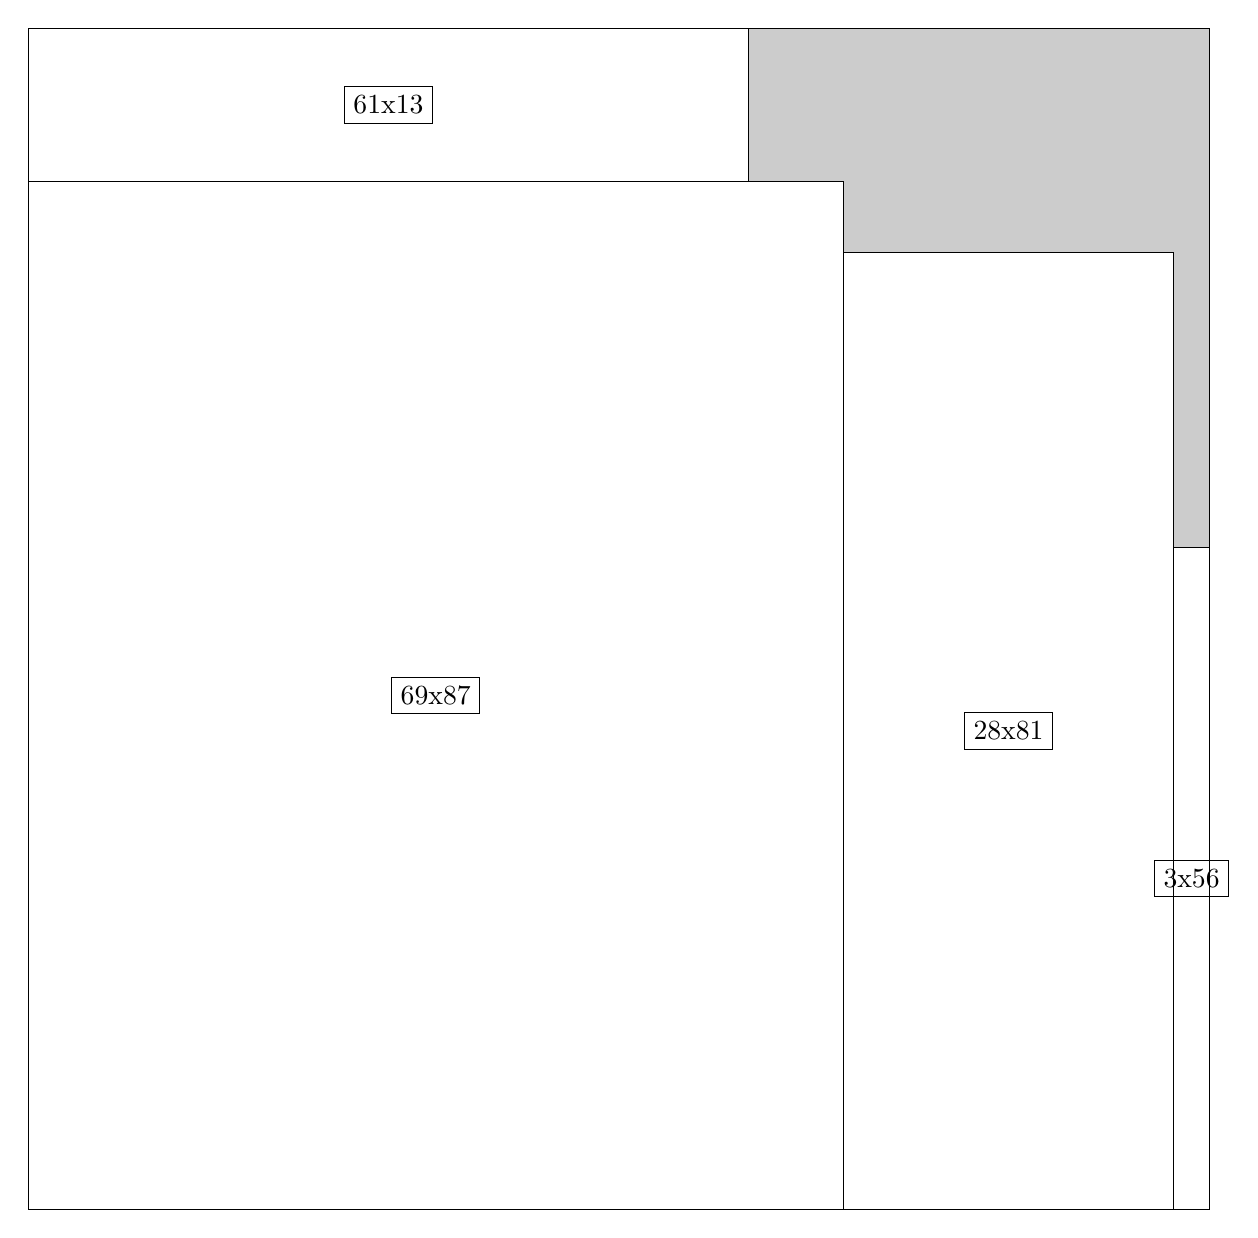
\begin{tikzpicture}[shorten >=1pt,scale=1.0,every node/.style={scale=1.0},->]
\tikzstyle{vertex}=[circle,fill=black!25,minimum size=14pt,inner sep=0pt]
\filldraw[fill=gray!40!white, draw=black] (0,0) rectangle (15.0,15.0);
\foreach \name/\x/\y/\w/\h in {69x87/0.0/0.0/10.35/13.049999999999999,28x81/10.35/0.0/4.2/12.15,61x13/0.0/13.049999999999999/9.15/1.95,3x56/14.549999999999999/0.0/0.44999999999999996/8.4}
\filldraw[fill=white!40!white, draw=black] (\x,\y) rectangle node[draw] (\name) {\name} ++(\w,\h);
\end{tikzpicture}


w =69 , h =87 , x =0 , y =0 , v =6003
\par
w =28 , h =81 , x =69 , y =0 , v =2268
\par
w =61 , h =13 , x =0 , y =87 , v =793
\par
w =3 , h =56 , x =97 , y =0 , v =168
\par
\newpage


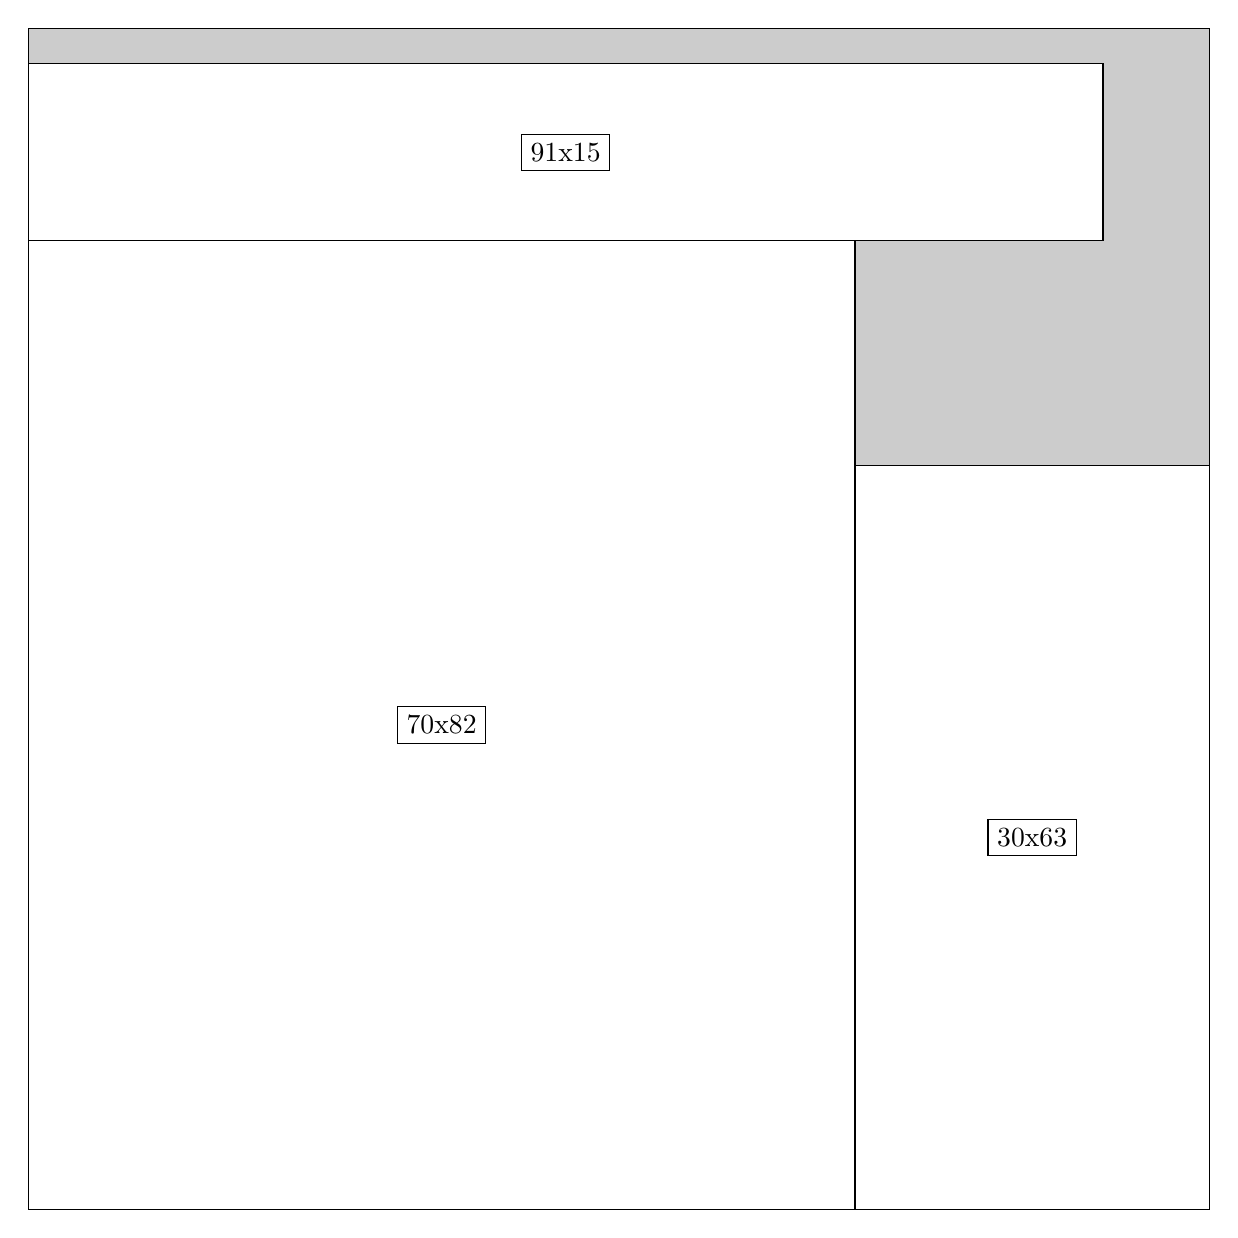
\begin{tikzpicture}[shorten >=1pt,scale=1.0,every node/.style={scale=1.0},->]
\tikzstyle{vertex}=[circle,fill=black!25,minimum size=14pt,inner sep=0pt]
\filldraw[fill=gray!40!white, draw=black] (0,0) rectangle (15.0,15.0);
\foreach \name/\x/\y/\w/\h in {70x82/0.0/0.0/10.5/12.299999999999999,30x63/10.5/0.0/4.5/9.45,91x15/0.0/12.299999999999999/13.65/2.25}
\filldraw[fill=white!40!white, draw=black] (\x,\y) rectangle node[draw] (\name) {\name} ++(\w,\h);
\end{tikzpicture}


w =70 , h =82 , x =0 , y =0 , v =5740
\par
w =30 , h =63 , x =70 , y =0 , v =1890
\par
w =91 , h =15 , x =0 , y =82 , v =1365
\par
\newpage


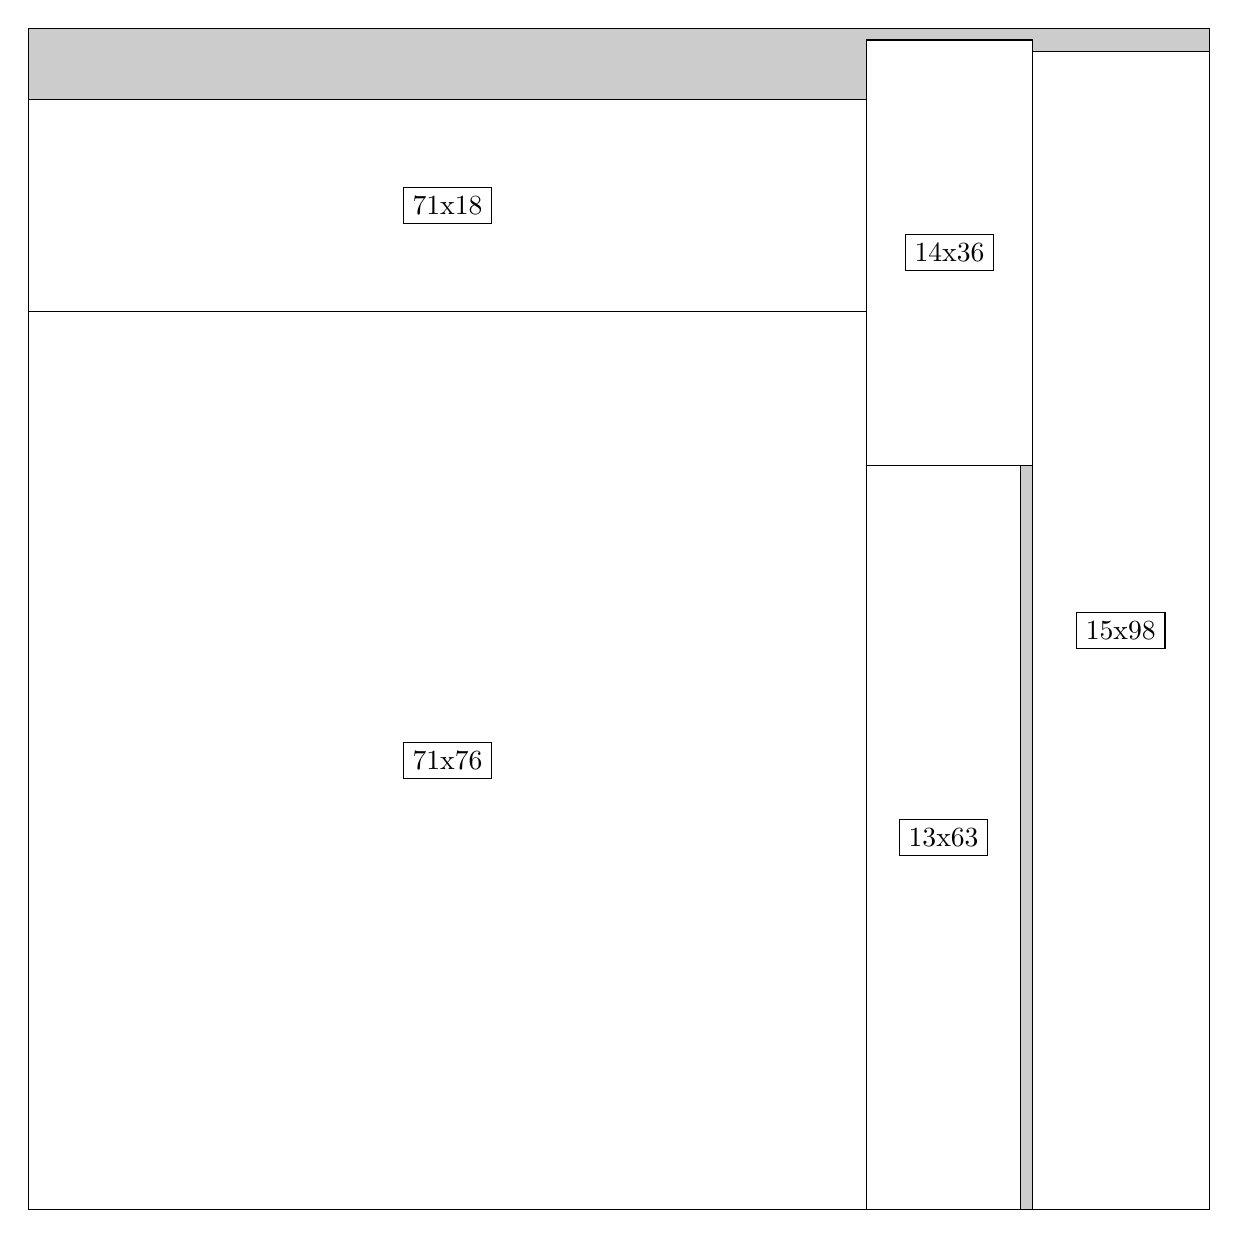
\begin{tikzpicture}[shorten >=1pt,scale=1.0,every node/.style={scale=1.0},->]
\tikzstyle{vertex}=[circle,fill=black!25,minimum size=14pt,inner sep=0pt]
\filldraw[fill=gray!40!white, draw=black] (0,0) rectangle (15.0,15.0);
\foreach \name/\x/\y/\w/\h in {71x76/0.0/0.0/10.65/11.4,15x98/12.75/0.0/2.25/14.7,71x18/0.0/11.4/10.65/2.6999999999999997,13x63/10.65/0.0/1.95/9.45,14x36/10.65/9.45/2.1/5.3999999999999995}
\filldraw[fill=white!40!white, draw=black] (\x,\y) rectangle node[draw] (\name) {\name} ++(\w,\h);
\end{tikzpicture}


w =71 , h =76 , x =0 , y =0 , v =5396
\par
w =15 , h =98 , x =85 , y =0 , v =1470
\par
w =71 , h =18 , x =0 , y =76 , v =1278
\par
w =13 , h =63 , x =71 , y =0 , v =819
\par
w =14 , h =36 , x =71 , y =63 , v =504
\par
\newpage


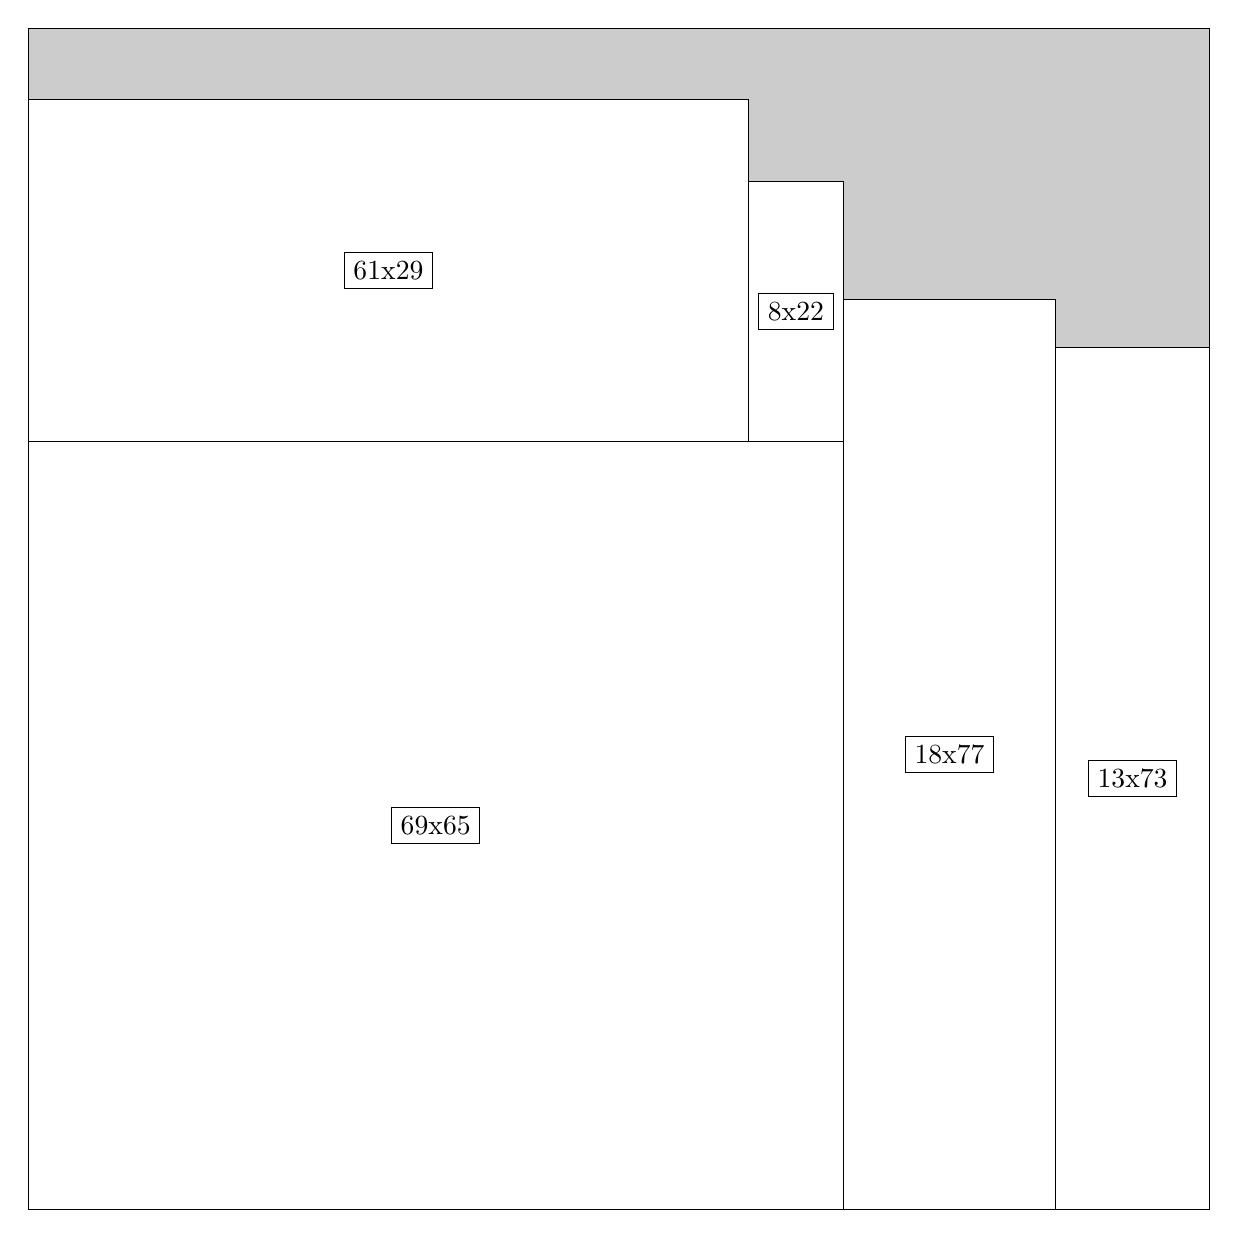
\begin{tikzpicture}[shorten >=1pt,scale=1.0,every node/.style={scale=1.0},->]
\tikzstyle{vertex}=[circle,fill=black!25,minimum size=14pt,inner sep=0pt]
\filldraw[fill=gray!40!white, draw=black] (0,0) rectangle (15.0,15.0);
\foreach \name/\x/\y/\w/\h in {69x65/0.0/0.0/10.35/9.75,61x29/0.0/9.75/9.15/4.35,18x77/10.35/0.0/2.6999999999999997/11.549999999999999,13x73/13.049999999999999/0.0/1.95/10.95,8x22/9.15/9.75/1.2/3.3}
\filldraw[fill=white!40!white, draw=black] (\x,\y) rectangle node[draw] (\name) {\name} ++(\w,\h);
\end{tikzpicture}


w =69 , h =65 , x =0 , y =0 , v =4485
\par
w =61 , h =29 , x =0 , y =65 , v =1769
\par
w =18 , h =77 , x =69 , y =0 , v =1386
\par
w =13 , h =73 , x =87 , y =0 , v =949
\par
w =8 , h =22 , x =61 , y =65 , v =176
\par
\newpage


\begin{tikzpicture}[shorten >=1pt,scale=1.0,every node/.style={scale=1.0},->]
\tikzstyle{vertex}=[circle,fill=black!25,minimum size=14pt,inner sep=0pt]
\filldraw[fill=gray!40!white, draw=black] (0,0) rectangle (15.0,15.0);
\foreach \name/\x/\y/\w/\h in {100x99/0.0/0.0/15.0/14.85}
\filldraw[fill=white!40!white, draw=black] (\x,\y) rectangle node[draw] (\name) {\name} ++(\w,\h);
\end{tikzpicture}


w =100 , h =99 , x =0 , y =0 , v =9900
\par
\newpage


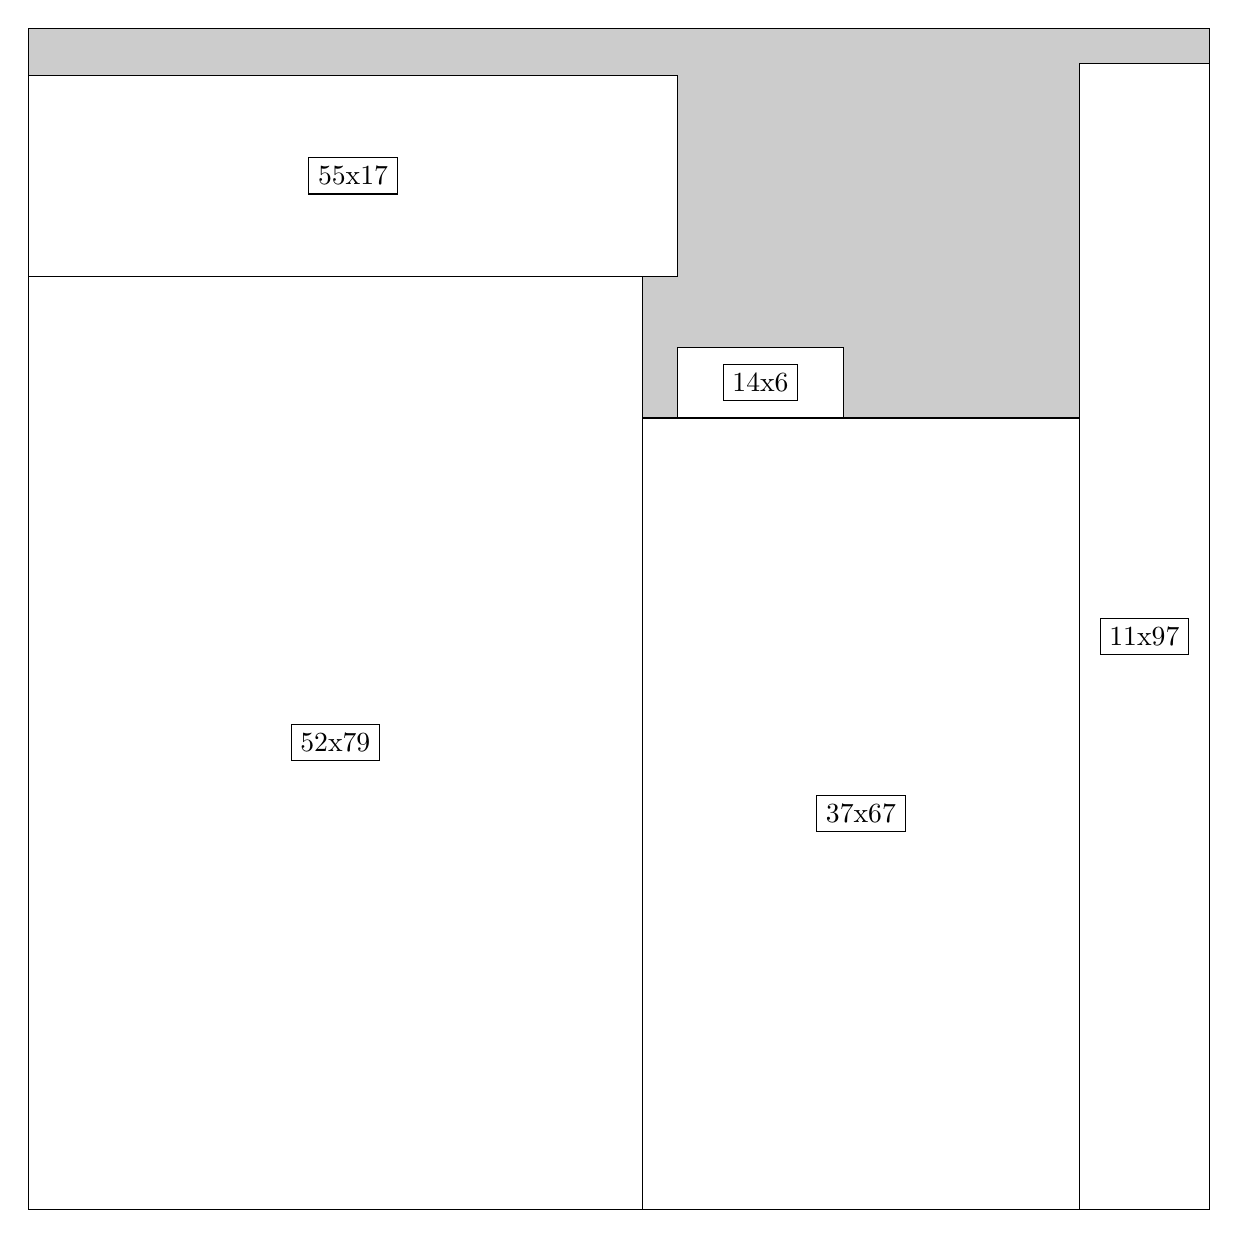
\begin{tikzpicture}[shorten >=1pt,scale=1.0,every node/.style={scale=1.0},->]
\tikzstyle{vertex}=[circle,fill=black!25,minimum size=14pt,inner sep=0pt]
\filldraw[fill=gray!40!white, draw=black] (0,0) rectangle (15.0,15.0);
\foreach \name/\x/\y/\w/\h in {52x79/0.0/0.0/7.8/11.85,37x67/7.8/0.0/5.55/10.049999999999999,11x97/13.35/0.0/1.65/14.549999999999999,55x17/0.0/11.85/8.25/2.55,14x6/8.25/10.049999999999999/2.1/0.8999999999999999}
\filldraw[fill=white!40!white, draw=black] (\x,\y) rectangle node[draw] (\name) {\name} ++(\w,\h);
\end{tikzpicture}


w =52 , h =79 , x =0 , y =0 , v =4108
\par
w =37 , h =67 , x =52 , y =0 , v =2479
\par
w =11 , h =97 , x =89 , y =0 , v =1067
\par
w =55 , h =17 , x =0 , y =79 , v =935
\par
w =14 , h =6 , x =55 , y =67 , v =84
\par
\newpage


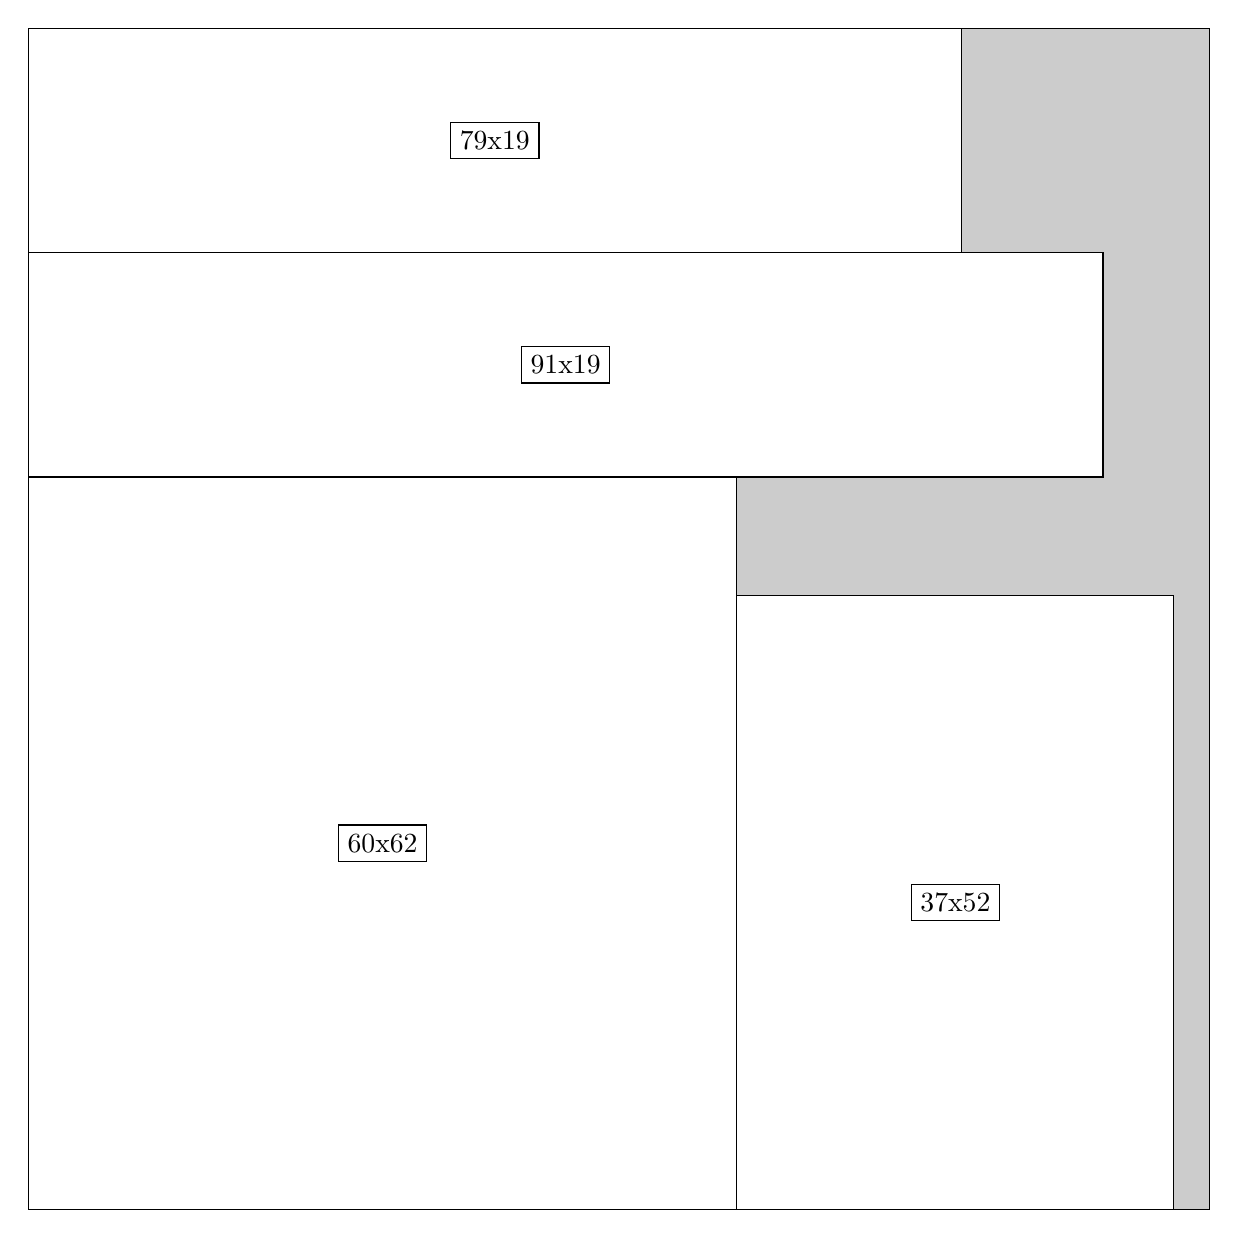
\begin{tikzpicture}[shorten >=1pt,scale=1.0,every node/.style={scale=1.0},->]
\tikzstyle{vertex}=[circle,fill=black!25,minimum size=14pt,inner sep=0pt]
\filldraw[fill=gray!40!white, draw=black] (0,0) rectangle (15.0,15.0);
\foreach \name/\x/\y/\w/\h in {60x62/0.0/0.0/9.0/9.299999999999999,37x52/9.0/0.0/5.55/7.8,91x19/0.0/9.299999999999999/13.65/2.85,79x19/0.0/12.15/11.85/2.85}
\filldraw[fill=white!40!white, draw=black] (\x,\y) rectangle node[draw] (\name) {\name} ++(\w,\h);
\end{tikzpicture}


w =60 , h =62 , x =0 , y =0 , v =3720
\par
w =37 , h =52 , x =60 , y =0 , v =1924
\par
w =91 , h =19 , x =0 , y =62 , v =1729
\par
w =79 , h =19 , x =0 , y =81 , v =1501
\par
\newpage


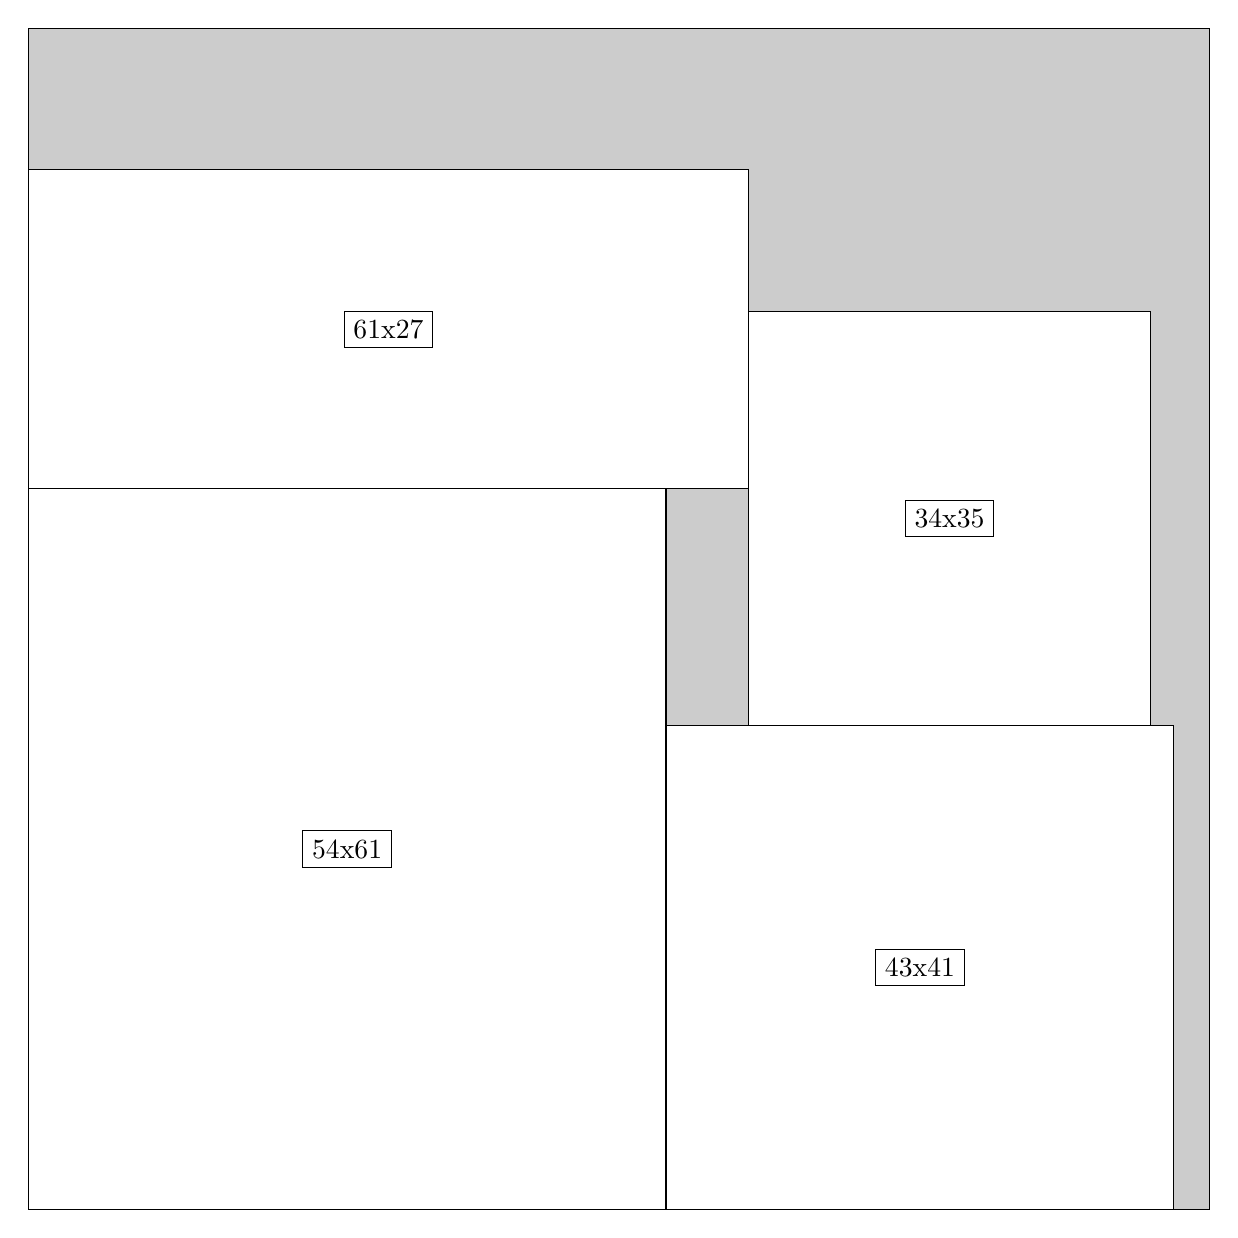
\begin{tikzpicture}[shorten >=1pt,scale=1.0,every node/.style={scale=1.0},->]
\tikzstyle{vertex}=[circle,fill=black!25,minimum size=14pt,inner sep=0pt]
\filldraw[fill=gray!40!white, draw=black] (0,0) rectangle (15.0,15.0);
\foreach \name/\x/\y/\w/\h in {54x61/0.0/0.0/8.1/9.15,43x41/8.1/0.0/6.45/6.1499999999999995,61x27/0.0/9.15/9.15/4.05,34x35/9.15/6.1499999999999995/5.1/5.25}
\filldraw[fill=white!40!white, draw=black] (\x,\y) rectangle node[draw] (\name) {\name} ++(\w,\h);
\end{tikzpicture}


w =54 , h =61 , x =0 , y =0 , v =3294
\par
w =43 , h =41 , x =54 , y =0 , v =1763
\par
w =61 , h =27 , x =0 , y =61 , v =1647
\par
w =34 , h =35 , x =61 , y =41 , v =1190
\par
\newpage


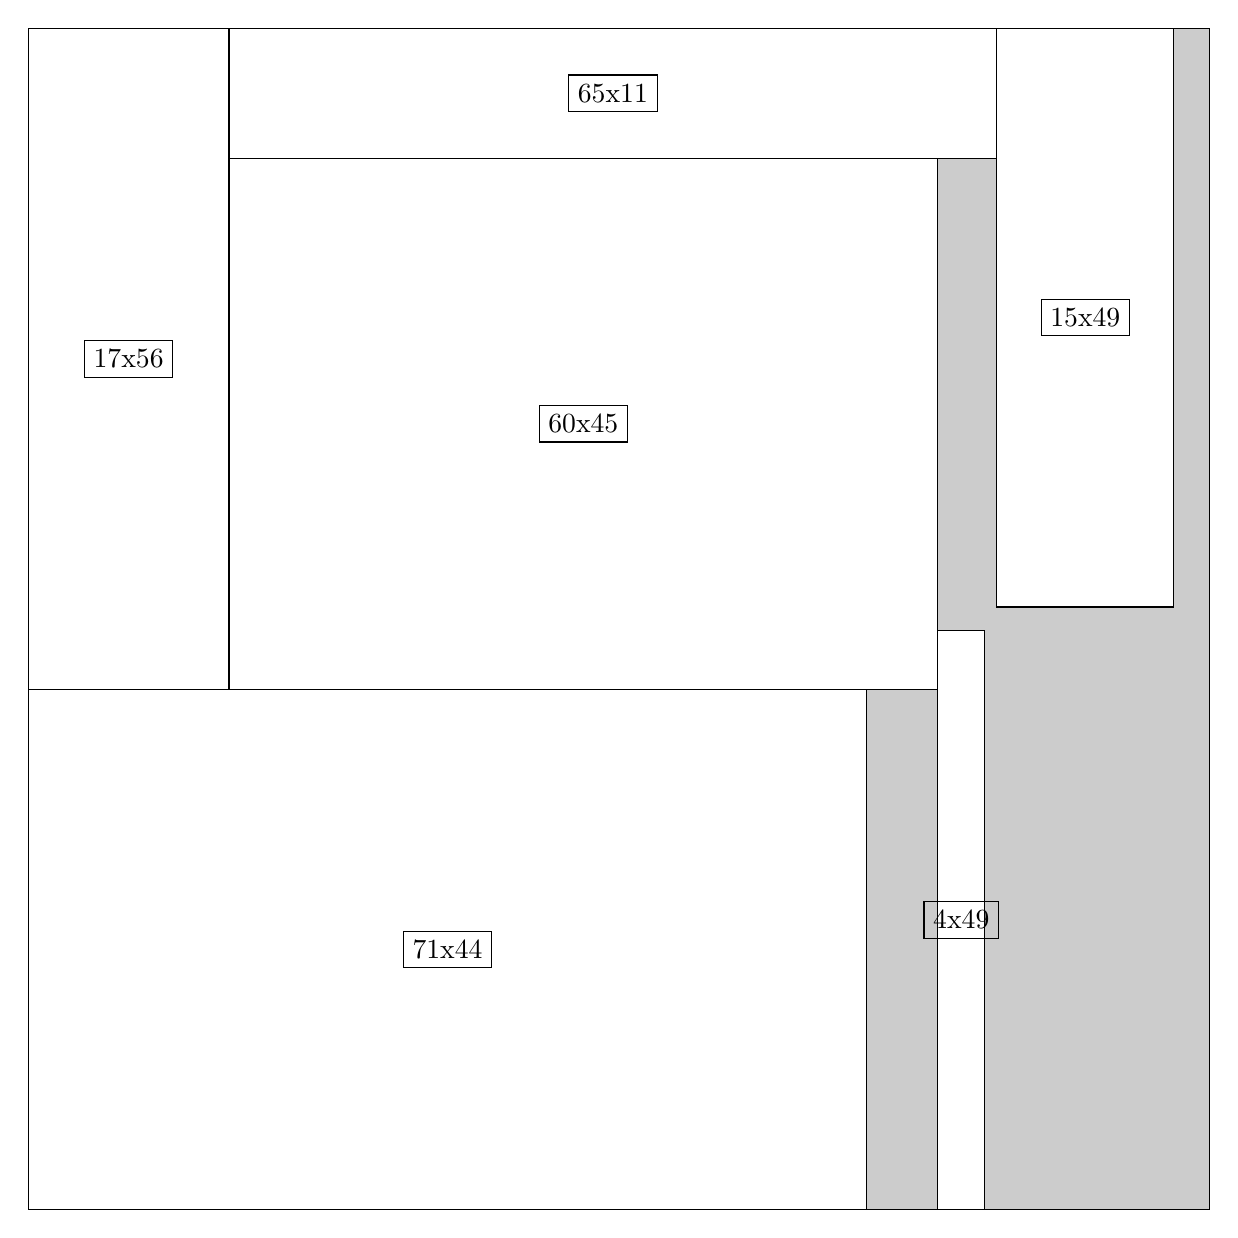
\begin{tikzpicture}[shorten >=1pt,scale=1.0,every node/.style={scale=1.0},->]
\tikzstyle{vertex}=[circle,fill=black!25,minimum size=14pt,inner sep=0pt]
\filldraw[fill=gray!40!white, draw=black] (0,0) rectangle (15.0,15.0);
\foreach \name/\x/\y/\w/\h in {71x44/0.0/0.0/10.65/6.6,60x45/2.55/6.6/9.0/6.75,17x56/0.0/6.6/2.55/8.4,15x49/12.299999999999999/7.6499999999999995/2.25/7.35,65x11/2.55/13.35/9.75/1.65,4x49/11.549999999999999/0.0/0.6/7.35}
\filldraw[fill=white!40!white, draw=black] (\x,\y) rectangle node[draw] (\name) {\name} ++(\w,\h);
\end{tikzpicture}


w =71 , h =44 , x =0 , y =0 , v =3124
\par
w =60 , h =45 , x =17 , y =44 , v =2700
\par
w =17 , h =56 , x =0 , y =44 , v =952
\par
w =15 , h =49 , x =82 , y =51 , v =735
\par
w =65 , h =11 , x =17 , y =89 , v =715
\par
w =4 , h =49 , x =77 , y =0 , v =196
\par
\newpage


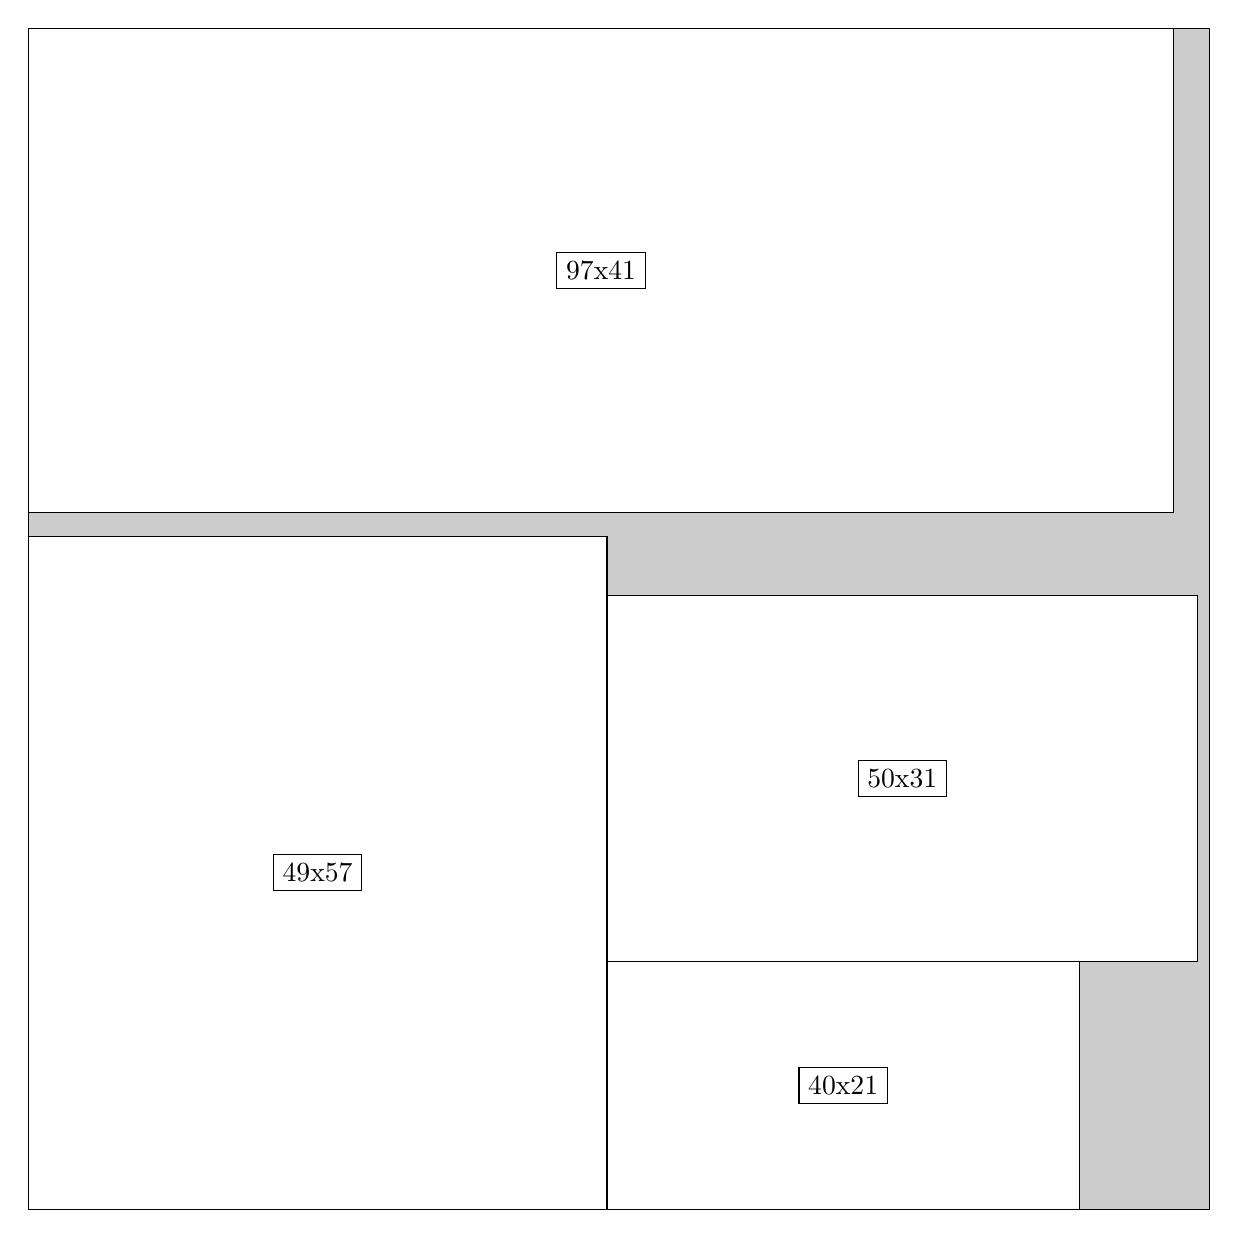
\begin{tikzpicture}[shorten >=1pt,scale=1.0,every node/.style={scale=1.0},->]
\tikzstyle{vertex}=[circle,fill=black!25,minimum size=14pt,inner sep=0pt]
\filldraw[fill=gray!40!white, draw=black] (0,0) rectangle (15.0,15.0);
\foreach \name/\x/\y/\w/\h in {97x41/0.0/8.85/14.549999999999999/6.1499999999999995,49x57/0.0/0.0/7.35/8.549999999999999,50x31/7.35/3.15/7.5/4.6499999999999995,40x21/7.35/0.0/6.0/3.15}
\filldraw[fill=white!40!white, draw=black] (\x,\y) rectangle node[draw] (\name) {\name} ++(\w,\h);
\end{tikzpicture}


w =97 , h =41 , x =0 , y =59 , v =3977
\par
w =49 , h =57 , x =0 , y =0 , v =2793
\par
w =50 , h =31 , x =49 , y =21 , v =1550
\par
w =40 , h =21 , x =49 , y =0 , v =840
\par
\newpage


\end{document}